%! TeX program = lualatex
\documentclass{tp}
\usepackage{chemfig}
\usepackage[version=4]{mhchem}
\usepackage{pgfplots}
\pgfplotsset{compat=1.17}
\usetikzlibrary{decorations.text}
\titre{TP23 : Dosages avec précipitation}
\begin{document}
%\small


\section{Objectif du TP}
 Dans ce TP, nous allons mettre en œuvre deux méthodes de dosage des ions \ce{Cl-} par précipitation : la méthode de \textsc{Mohr} (dosage direct) et la méthode de \textsc{Charpentier-Volhard} (dosage indirect).

\section{Indicateurs colorés}%
\label{sec:indicateurs_colores}

Il s'agit ici d'effectuer des tests en tube à essais de manière à justifier les choix d'indicateurs colorés des deux dosages auxquels on va s'intéresser.

\subsection{Méthode de \textsc{Mohr} : étude de la compétition entre précipités}%
\label{sub:methode_de_mohr_etude_de_la_competition_entre_precipites}

\begin{itemize}
  \item \textbf{Test n\no 1} : à \SI{1}{\milli\litre} de chromate de potassium (\ce{2K+ + CrO4^2-}), ajouter quelques gouttes de nitrate d'argent. Observer et conclure. Écrire l'équation de la réaction et calculer sa constante d'équilibre.

  \item \textbf{Test n\no 2} : dans un autre tube à essais, introduire \SI{0.5}{\milli\litre} de chlorure de sodium et \SI{0.5}{\milli\litre} de chromate de potassium ; ajouter goutte à goutte le nitrate d'argent. Observer et conclure. Écrire l'équation de la réaction et calculer sa constante d'équilibre. Justifier pourquoi c'est cette réaction qu'on observe.
\end{itemize}

\textit{Données : }$\pKs(\ce{Ag2CrO4(s)})=12$ ; $\pKs(\ce{AgCl(s)})=\num{9.8}$ 

\subsection{Méthode de \textsc{Charpentier-Volhard} : test impliquant une réaction de complexation}%
\label{sub:methode_de_charpentier_volhard_test}

\textit{Les réactions de complexation ne sont pas au programme, on donne ici le résultat du test caractéristique qui sera utilisé par la suite}

Si à \SI{1}{\milli\litre} de chlorure de fer (III) (\ce{Fe^3+ + 3Cl-}) on ajoute une goutte de thiocyanate de potassium (\ce{K+ + SCN-}), la solution se teinte d'une couleur rouge très intense tout en restant transparente ; il y a formation du complexe \ce{FeSCN^2+} selon la réaction :
\begin{equation}
  \ce{Fe^3+(aq) + SCN-(aq) <=> FeSCN^2+(aq)}
\end{equation}
de constante d'équilibre $\beta_1$.
Cette expérience constitue un test caractéristique de la présence des ions \ce{Fe^3+}.

\section{Dosage des ions chlorure par la méthode de \textsc{Mohr} }%
\label{sec:dosage_des_ions_chlorure_par_la_methode_de_mohr_}

Le but du dosage est de déterminer la concentration inconnue $c_0$ en ions \ce{Cl-} d'une solution de sérum physiologique (solution de chlorure de sodium (\ce{Na+ + Cl-})).

\textbf{Solution titrée : } $V_0=\SI{5}{\milli\litre}$ de sérum physiologique de concentration $c_0$ en ions chlorure $+$ \SI{20}{\milli\litre} d'eau distillée.

\textbf{Solution titrante : } Solution de nitrate d'argent de concentration $c=\SI{5e-2}{\mol\per\litre}$, de volume $V$ versé.

\begin{itemize}
  \item Écrire la réaction de dosage et calculer sa constante d'équilibre. Cette réaction présente-t-elle toutes les caractéristiques d'une réaction de dosage.

  \item Quelle est la relation à l'équivalence

  \item Faut-il mesurer précisément les \SI{20}{\milli\litre} d'eau distillée présents dans la solution titrée ?
\end{itemize}
Afin de repérer l'équivalence, on utilise comme indicateur coloré le chromate de potassium (10 gouttes à \SI{1}{\mol\per\litre}). Quel est le changement de couleur de la solution contenue dans le bécher lors du dosage.

\begin{itemize}
  \item Réaliser le dosage. Conserver le nitrate d'argent restant dans la burette pour la suite du TP. 

  \item Calculer la concentration inconnue $c_0$ du sérum physiologique.

  \item Le sérum physiologique est une solution aqueuse de \ce{NaCl} de concentration massique égale à \SI{9}{\gram\per\litre}. Vos résultats sont-ils compatibles avec cette valeur ? ($M(\ce{Na})=\SI{23}{\gram\per\mol}$ et $M(\ce{Cl})=\SI{35.5}{\gram\per\mol}$) 
\end{itemize}

\textbf{Attention : } Il existe des limites à la méthode de Mohr. Si le milieu est trop acide, il se produirait la réaction de protonation de l'ion chromate qui produit l'ion \ce{HCrO4-} qui ne précipite pas avec les ions \ce{Ag+}. Si par ailleurs le milieu est trop basique, il y aurait apparition des précipités \ce{AgOH} ou encore \ce{Ag2O} qui fausseraient le dosage.

\section{Dosage des ions chlorure par la méthode de \textsc{Charpentier-Volhard}}%
\label{sec:dosage_des_ions_chlorure_par_la_methode_de_charpentier-volhard}

\subsection{Principe de la méthode}%
\label{sub:principe_de_la_methode}
La méthode de \textsc{Charpentier-Volhard} est un \emph{dosage en retour}. Au lieu de doser directement les ions \ce{Cl-}, on les fait réagir avec un excès d'ions \ce{Ag+} puis on dose les \ce{Ag+} restants par un solution de \ce{SCN-} en présence de nitrate de fer (III) utilisé comme indicateur coloré.

\begin{itemize}
  \item Écrire la réaction de dosage et calculer sa constante d'équilibre.
\end{itemize}

\textit{Données  : } $\log(\beta_1)=\num{2.2}$ ; $\pKs(\ce{AgSCN})=12$.  

Schématisation du dosage
\begin{center}
  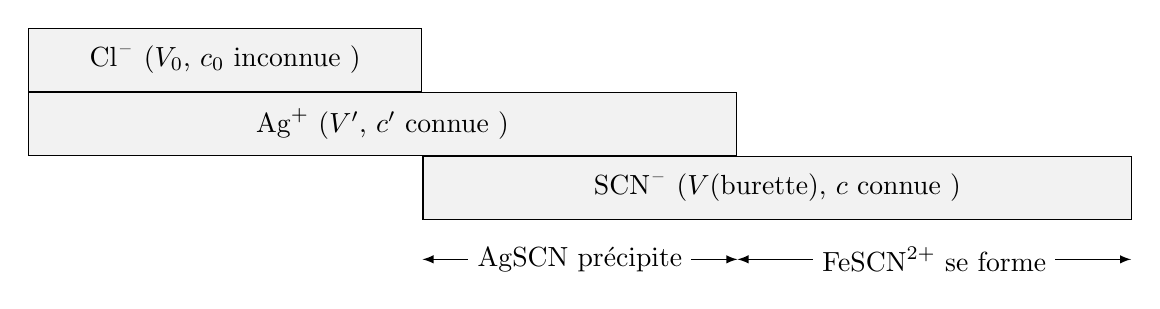
\begin{tikzpicture}
    \node[above right, rectangle, draw, fill=gray!10, minimum width=5cm, minimum height=0.8cm](Cl) at (0,0) {\ce{Cl-} ($V_0$, $c_0$ inconnue )};
    \node[below right, rectangle, draw, fill=gray!10, minimum width=9cm, minimum height=0.8cm](Ag) at (Cl.south west) {\ce{Ag+} ($V'$, $c'$ connue )};
    \node[below right, rectangle, draw, fill=gray!10, minimum width=9cm, minimum height=0.8cm](SCN) at (Cl.south east|-Ag.south) {\ce{SCN-} ($V$(burette), $c$ connue )};

    \draw[latex-latex] (SCN.south west) ++(0, -0.5) -- node[fill=white]{\ce{AgSCN} précipite} ++(4,0) coordinate (B);
    \draw[latex-latex] (B) -- node[fill=white]{\ce{FeSCN^2+} se forme} ++(5, 0);
  \end{tikzpicture}
\end{center}

\subsection{Dosage}%
\label{sub:dosage}

\begin{itemize}
  \item Récupérer le reste de nitrate d'argent contenu dans la burette et \textbf{bien la rincer} à l'eau distillée.

  \item Placer dans la burette \SI{10}{\milli\litre} d'une solution de concentration $c = \SI{5.0e-2}{\mol\per\litre}$ de thiocyanate de potassium.  

  \item Placer dans un erlenmeyer un volume $V_0 = \SI{25.0}{\milli\litre}$ d'eau minérale de concentration $c_0$ en ions \ce{Cl-} et $V'= \SI{10}{\milli\litre}$ de solution de nitrate d'argent de concentration $c'= \SI{5.0e-2}{\mol\per\litre}$. Bien agiter jusqu'à ce que le précipité soit bien rassemblé. Ajouter \SI{25}{\milli\litre} d'acide nitrique\footnote{L'acide nitrique sert à se placer en milieu acide, pour optimiser la précipitation de \ce{AgCl}. On empêche ainsi l'apparition des précipités \ce{Fe(OH)3 (s)} et \ce{Ag2O (s)}}.

\item Filtrer avec soin la solution en rinçant le précipité à l'eau distillée. Ne pas oublier de rajouter les eaux de lavage au filtrat.

\item Ajouter au filtrat \SI{1}{\milli\litre} (15 gouttes) de l'indicateur coloré (alun ferrique).

\item Réaliser le dosage du filtrat.

\item Déduire la concentration $c_0$ en ions chlorure de l'eau minérale, comparer à l'étiquette de la bouteille.

\end{itemize}

\end{document}

